\documentclass{report}
\usepackage[fontsize=13pt]{scrextend}

\usepackage{my_lab}

\begin{document}

\graphicspath{{figures}}

\MiptLabTitle{4.3.2}{Дифракция света на ультразвуковой волне в жидкости}

\begin{document}
\textbf{Цель:} изучение дифракции света на синусоидальной акустической решётке и наблюдение фазовой решётки методом тёмного
поля.

\textbf{Используются в работе:} оптическая скамья, осветитель, два длиннофокусных объектива, кювета с жидкостью, кварцевый излучатель
с микрометрическим винтом, генератор ультразвуковой частоты, линза, вертикальная нить на рейтере, микроскоп.

\section*{Установка}
Схема установки приведена на рисунке \ref{shema1}. Источник света Л через светофильтр Ф и
конденсор К освещает вертикальную щель $ S $, находящуюся в фокусе объектива $
O_1 $. После объектива параллельный световой пучок проходит через кювету С
перпендикулярно акустической решетке, и дифракционная картина собирается в
фокальной плоскости объектива $ O_2 $ , наблюдается при помощи микроскопа М.


\begin{figure}[h!]
	\centering
	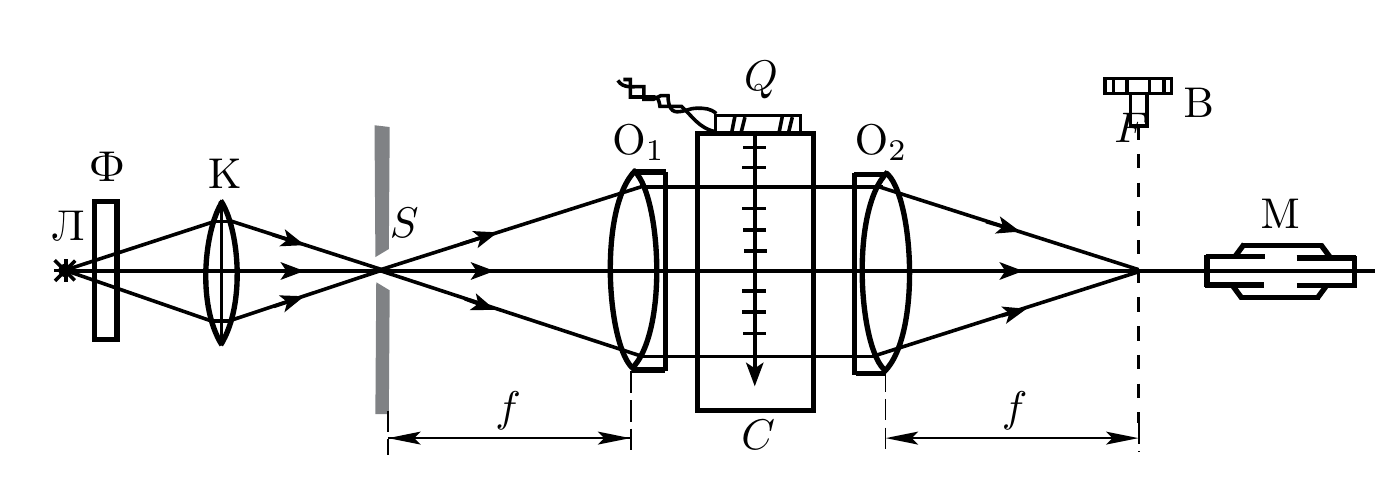
\includegraphics[width=0.7\textwidth]{figures/shema1.png}
	\caption{Схема для наблюдения дифракции на акустической решетке}
	\label{shema1}
\end{figure}

Измерим положения дифракционных максимумов с помощью микроскопического винта B.

Для наблюдения акустической решетки используется метод темного поля, который
заключается в устранении центрального дифракционного максимума с помощью
непрозрачного экрана.

\begin{figure}[h!]
	\centering
	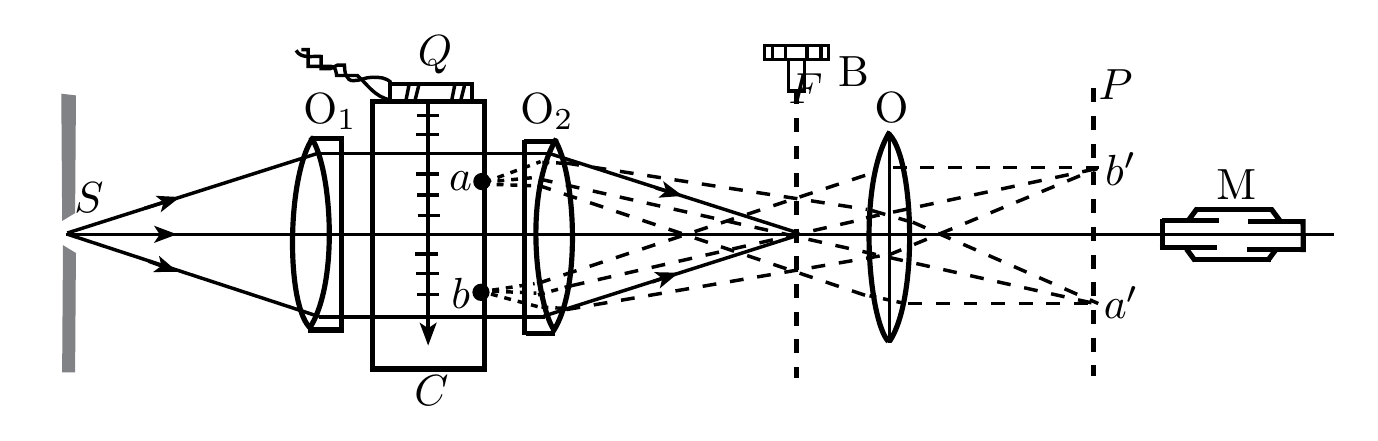
\includegraphics[width=0.7\textwidth]{shema2.png}
	\caption{Схема для наблюдения дифракции методом темного поля}
	\label{shema2}
\end{figure}

\section*{Теоретическая часть}

\begin{equation}\label{}
	n = n_0 (1 + m \cos \Omega x)
\end{equation}

\begin{equation}\label{}
	\phi  = k n L = \phi_0 (1 + m \cos \Omega x)
\end{equation}

\begin{equation}\label{}
	\Lambda \sin \theta_m = m \lambda
\end{equation}

\begin{equation}\label{}
	\Lambda = m \lambda F/ l_m
\end{equation}

\begin{equation}\label{}
	v = \Lambda \nu
\end{equation}

\section{Ход работы}
\section{Выводы}
\end{document}
